\documentclass[
aspectratio=169 % comment for 4:3
]{beamer}

\newcommand{\cmd}[1]{\texttt{\textbf{#1}}}
\newcommand{\args}[1]{\texttt{\textit{#1}}}

\usetheme[
hidetotal, % hide the total number of slides on the bottom right
hidenumbers, % hide current slide number
% hidename, % hide author name and title in footline
hidebullets, % use empty bullets in itemize
hidefootline, % hide the footline
%
% the previous options allow for a minimalistic style as recommended by Patrick
% Winston in his "how to speak" lecture at MIT
%
% sidebar, % show sidebar
hugetitle, % print main title in huge font
% thin, % use a thinner font
% bold, % use bold titles
% standardtitle, % use standard title slide (no picture)
]{mfrancois}

\setsecondarylogo{title/isia-logo} % Add a secondary logo to the title slide, optional
\settitleimage{title/raspberry} % Change the title slide image, optional (use images with a ratio identical to the one provided)

\author[F. Marelli]{François Marelli}
\affiliation[UMONS]{UMONS, ISIA Lab}
\title{Atelier Créactifs: Raspberry Pi}
\subtitle{Séance 2: Le terminal}
\extras{
\includegraphics[height=25pt]{title/creactifs}}
\date{9 février 2026}

\graphicspath{{images}}

\begin{document}

\maketitle

\begin{frame}{Des problèmes courants}{Quand on commence à utiliser un Raspberry
        Pi}

    Que faire quand:
    \begin{itemize}
        \item vous n'avez pas d'accès physique au Raspberry Pi
        \item l'outil graphique des paramètres système ne suffit pas
        \item des tâches simples sont répétitives et ennuyeuses
        \item les ressources doivent être économisées
        \item vous devez vous débrouiller avec un système Linux inconnu
    \end{itemize}

    \bigskip Une solution commune: \alert{le terminal!
    }
\end{frame}

\begin{frame}{Plan de la séance}
    \tableofcontents
\end{frame}

\section{C'est quoi un terminal?}
\frame{\sectionpage}

\begin{frame}{Une interface de contrôle basée sur du texte}{C'est moche, mais
        efficace}

    CLI (Command Line Interface) >< GUI (Graphical User Interface)
    \begin{itemize}
        \item \(\rightarrow\) Pas d'interface graphique = pas de fenêtres,
              boutons ou souris!
    \end{itemize}

    \bigskip

    Interface ancienne mais encore utilisée car elle:

    \begin{itemize}
        \item utilise peu de ressources
        \item donne accès à des outils système puissants
        \item permet d'automatiser des tâches
        \item permet de contrôler une machine à distance
        \item est disponible universellement indépendamment de l'interface
              graphique
    \end{itemize}
\end{frame}

\begin{frame}{Premiers pas} 4 options pour ouvrir un terminal:
    \begin{itemize}
        \item cliquer sur l'icône du terminal dans la barre d'outils
        \item utiliser le menu principal
        \item utiliser un raccourci clavier: \texttt{Ctrl+Alt+T}
        \item changer de terminal virtuel avec \texttt{Ctrl+Alt+Fn} (bouée en
              cas de plantage GUI)
    \end{itemize}

    \bigskip

    L'invite de commande (prompt):
    \texttt{\alert<2>{rpi}@\alert<3>{rpi-01}:\alert<4>{\textasciitilde} \$}
    \begin{itemize}
        \item<2-> \texttt{\alert<2>{rpi}}: nom de l'utilisateur

        \item<3-> \texttt{\alert<3>{rpi-01}}: nom de l'hôte

        \item<4-> \texttt{\alert<4>{\textasciitilde}}: répertoire courant
        (\textasciitilde = home)
    \end{itemize}

\end{frame}

\begin{frame}{Anatomie d'une commande}

    Une commande = un programme + des options + des arguments

    \bigskip

    \texttt{\textbf{ls} -l Documents}

    \begin{itemize}
        \item \texttt{ls}: nom de la commande (list)
        \item \texttt{-l}: option
        \item \texttt{Documents}: argument ("entrée" principale de la commande)
    \end{itemize}

    \bigskip \cmd{ls} sans arguments pour une liste simple du répertoire courant

    \bigskip \alert{Tip:} utiliser \texttt{Tab} pour compléter les commandes et
    les chemins

\end{frame}

\begin{frame}{La sortie de \texttt{ls}}{Liste le contenu d'un répertoire} Par
    colonne:
    \begin{enumerate}
        \item  type et permissions d'accès
        \item nombre de liens vers cet élément
        \item utilisateur propriétaire
        \item groupe propriétaire
        \item taille en octets
        \item date de dernière modification
        \item nom du fichier ou du répertoire
    \end{enumerate}
\end{frame}

\begin{frame}{Intérpréter les permissions}{Commande: \cmd{ls -l}}

    1 lettre + 3 groupes de 3:

    \smallskip\texttt{d rwx r-x r-x}

    \bigskip

    \begin{enumerate}
        \item \texttt{d}: type (d = dossier, - = fichier, l = lien)
        \item \texttt{rwx}: permissions du propriétaire
        \item \texttt{r-x}: permissions du groupe
        \item \texttt{r-x}: permissions des autres utilisateurs
    \end{enumerate}

    \bigskip Permissions: r = lecture, w = écriture, x = exécution, - = pas de
    permission

    \medskip Exécution pour un dossier = accès au contenu

\end{frame}

\section{Naviguer dans le système de fichiers} \frame{\sectionpage}

\begin{frame}{S'orienter dans les répertoires}{Tous les chemins mèment à home}

    \cmd{pwd} (print working directory): afficher le \textit{chemin} du
    répertoire courant

    \bigskip 2 types de chemins:
    \begin{itemize}
        \item absolu: commence par \texttt{/} et explicite depuis la racine
        \item relatif: à partir du répertoire courant
    \end{itemize}

    \bigskip Exemple:
    \begin{itemize}
        \item \texttt{/home/rpi/Documents} - absolu
        \item \texttt{Documents} - relatif (équivalent si on est dans
              \texttt{/home/rpi})
    \end{itemize}

    \bigskip \alert{Tip:} contrairement à Windows, les chemins utilisent
    \texttt{/} et non \texttt{\textbackslash}

\end{frame}

\begin{frame}[fragile]{Se déplacer dans les répertoires}

    \cmd{cd}\args{ chemin} (change directory): se déplacer
    vers le chemin spécifié

    \bigskip
    Chemins relatifs locaux:

    \bigskip
    \begin{tabular}{rrll}
         & \texttt{.}  & = & répertoire courant \\
         & \texttt{..} & = & répertoire parent
    \end{tabular}

    \bigskip
    Exemple:

    \begin{lstlisting}
    $ cd
    $ cd ./Documents
    $ cd ../Desktop
    \end{lstlisting}

    \bigskip
    \alert{Tip:} \cmd{cd} sans argument = retour au home

\end{frame}

\begin{frame}[fragile]{La racine}{I am root}
    \texttt{/} (root):
    \begin{itemize}
        \item est à l'origine de tous les chemins absolus
        \item est un répertoire comme les autres
        \item contient l'entièreté du système de fichiers
    \end{itemize}

    \bigskip
    Que contient la racine?

    \begin{lstlisting}
    $ cd /
    $ ls -l
    \end{lstlisting}

    \alert{Tip:} \textit{root} est le nom du super-utilisateur (administrateur)
\end{frame}

\begin{frame}{L'arbre de dossiers Linux}{Les principaux répertoires}
    \begin{itemize}
        \item \texttt{/home}: répertoires personnels des utilisateurs
        \item \texttt{/root}: répertoire personnel de l'utilisateur root
        \item \texttt{/etc}: configuration du système
        \item \texttt{/boot}: fichiers utiles au démarrage du système
        \item \texttt{/bin} et \texttt{/sbin}: exécutables (binaires),
              programmes
        \item \texttt{/lib}: librairies partagées (code réutilisable pour les
              programmes)
        \item \texttt{/opt}: logiciels additionnels hors standard
        \item \texttt{/media} et \texttt{/mnt}: points de montage pour les
              périphériques de stockage
        \item \texttt{/tmp}: fichiers temporaires (supprimés régulièrement)
    \end{itemize}
\end{frame}

\begin{frame}{L'arbre de dossiers Linux}{Les autres répertoires}
    \begin{itemize}
        \item \texttt{/usr}: ressources partagées (quasiment tout ce qui est
              installé)
        \item \texttt{/dev}: périphériques (interfaces vers le matériel)
        \item \texttt{/lost+found}: données récupérées après une erreur de
              disque
        \item \texttt{/proc} et \texttt{/sys}: état du système et des processus
              en cours
        \item \texttt{/run}: informations sur les tâches en cours
        \item \texttt{/srv}: données pour les services fournis par le système
        \item \texttt{/var}: variables qui changent régulièrement
              (logs, données d'applicaions)
    \end{itemize}

    \bigskip
    Exemple: \texttt{/proc/cpuinfo} contient des informations sur le processeur

\end{frame}

\begin{frame}{Le répertoire home}{Home sweet home}
    Retour au home, lister le répertoire avec \texttt{\textbf{ls} -la}
    \bigskip

    Principaux fichiers et dossiers cachés:
    \begin{itemize}
        \item \texttt{.profile}: script exécuté à la connexion d'une session
        \item \texttt{.bashrc}: script exécuté à l'ouverture d'un terminal
        \item \texttt{.bash\textunderscore history}: historique du terminal
        \item \texttt{.config}: fichiers de configuration locaux
        \item \texttt{.cache}: cache et données des applications locales
        \item \texttt{.local}: équivalent de \texttt{/usr} pour les fichiers et
              programmes locaux
    \end{itemize}

    \bigskip
    \alert{Tip:} tout fichier ou dossier dont le nom commence par \texttt{.} est
    caché

\end{frame}

\begin{frame}{Déplacer des fichiers}
    \cmd{mkdir}\args{ nom\_dossier} (make directory): créer un nouveau dossier
    \smallskip

    \cmd{mv}\args{ source destination} (move): déplacer/renommer un fichier ou
    un dossier
    \smallskip

    \cmd{cp}\args{ source destination} (copy): copier un fichier
    \smallskip

    \cmd{rm}\args{ fichier} (remove): supprimer un fichier,
    \textit{définitivement!}

    \bigskip
    Excercice:
    \begin{enumerate}
        \item déplacez-vous où vous avez crée votre fichier texte avec vos noms
        \item créez un sous-dossier et copiez le fichier dans ce sous-dossier
        \item vérifiez que la manipulation a marché avec l'interface graphique
        \item supprimez ce dossier
    \end{enumerate}
    \bigskip

    \alert{Tip:} \cmd{cp} et \cmd{rm} ont besoin de l'option \texttt{-r}
    (récursif) pour les dossiers
\end{frame}

\begin{frame}{Afficher le contenu d'un fichier}
    \cmd{cat}\args{ fichier} : afficher le contenu d'un fichier
    \bigskip

    \cmd{less}\args{ fichier} : afficher le contenu d'un fichier
    page par page, avec navigation
    \begin{itemize}
        \item flèches pour se déplacer ligne par ligne
        \item \texttt{espace} pour avancer d'une page
        \item \texttt{b} pour reculer d'une page
        \item \texttt{q} pour quitter
    \end{itemize}
    \bigskip

    \cmd{cat} est plus simple, mais \cmd{less} est plus pratique
    pour les fichiers longs

    \bigskip
    \alert{Tip:} utiliser \texttt{Ctrl+C} pour interrompre une commande en cours
    (ex: \cmd{cat} sans argument)
\end{frame}

\begin{frame}{Modifier un fichier}
    \cmd{nano}\args{ fichier} : éditeur de texte en ligne de commande
    \begin{itemize}
        \item flèches pour naviguer
        \item \texttt{Ctrl+O} pour enregistrer
        \item \texttt{Ctrl+X} pour quitter
    \end{itemize}
    \bigskip

    \alert{Tip:} il existe d'autres éditeurs plus avancés (vim, emacs), mais
    nano est plus simple pour débuter et souvent disponible par défaut
\end{frame}

\begin{frame}{Exercice de synthèse}{Édition et affichage de fichiers texte}

    \begin{enumerate}
        \item créez un fichier texte avec \cmd{nano}
        \item collez 30 paragraphes de \textit{Lorem ipsum} dans ce
              fichier\\
              \href{https://loremipsum.io/generator
                  /?n=30\&t=p}{https://loremipsum.io/generator/}
        \item affichez le contenu de ce fichier avec \cmd{cat}
        \item affichez le contenu de ce fichier avec \cmd{less}
    \end{enumerate}

    \bigskip
    \alert{Tip:} \texttt{Ctrl+C} et \texttt{Ctrl+V} pour copier/coller
    sont remplacés par \texttt{Ctrl+Shift+C} et \texttt{Ctrl+Shift+V} dans le
    terminal!
\end{frame}

\section{Des outils pour se simplifier la vie} \frame{\sectionpage}

\begin{frame}{Gérer les processus en cours}
    \cmd{htop}: gestionnaire des tâches dans le terminal (\texttt{q} pour
    quitter)

    \bigskip
    Affiche:
    \begin{itemize}
        \item utilisation du CPU et de la mémoire
        \item temps d'activité du système
        \item numéro du processus (PID) et utilisateur responsable du processus
        \item temps d'exécution
        \item commande associée au processus
    \end{itemize}

    \bigskip
    Permet de tuer un processus avec \texttt{F9} (\texttt{SIGKILL})

    \bigskip
    Exercice: ouvrez le navigateur web, vérifiez l'impact en ressources puis
    tuez le processus
\end{frame}

\begin{frame}{Mettre à jour le système}
    \cmd{apt} (Advanced Package Tool): gestionnaire de paquets de Raspberry Pi
    OS

    \smallskip
    Un \textit{paquet} peut contenir un programme, une librairie, des données

    \bigskip
    Utilisé avec une sous-commande:
    \begin{itemize}
        \item \texttt{update}: met à jour la liste des paquets disponibles
        \item \texttt{upgrade}: met à jour les paquets installés
        \item \texttt{install}\args{ paquet}: installe un paquet
        \item \texttt{remove}\args{ paquet}: désinstalle un paquet
    \end{itemize}

    \bigskip
    \alert{Tip:} certaines commandes comme \cmd{apt} nécessitent les droits
    d'administrateur
\end{frame}

\begin{frame}[fragile]{Les pleins pouvoirs}{Un grand pouvoir implique de grandes
        responsabilités}
    \cmd{sudo} (superuser do): exécuter ce qui suit avec les droits
    d'administrateur

    \smallskip
    \(\rightarrow\) donne temporairement les mêmes permissions que \textit{root}

    \bigskip
    Mettre à jour le système:
    \begin{lstlisting}
    $ sudo apt update
    $ sudo apt upgrade
    \end{lstlisting}

    \begin{alertblock}{Le danger de \cmd{sudo}}
        Avec les permissions de \textit{root}, on peut causer des dégâts
        considérables

        \smallskip
        Par exemple, ne \textbf{JAMAIS} faire: \texttt{\textbf{sudo rm} -rf /},
        cela supprimerait tout le système!
    \end{alertblock}
\end{frame}

\begin{frame}[fragile]{Un explorateur de fichiers en ligne de commande}

    \cmd{ranger} est un explorateur de fichiers visuel dans le terminal
    \begin{itemize}
        \item flèches pour naviguer
        \item \texttt{Enter} ou \(\rightarrow\) pour ouvrir un fichier ou entrer
              dans un dossier
        \item \texttt{Shift+S} pour ouvrir un terminal dans le dossier courant
        \item \texttt{q} pour quitter
        \item \texttt{:help} pour ouvrir un menu d'aide
    \end{itemize}

    \bigskip
    \cmd{ranger} n'est pas installé par défaut:
    \begin{lstlisting}
    $ sudo apt install ranger
    $ ranger
    \end{lstlisting}

    Exercice: retrouvez et visualisez votre fichier \textit{Lorem ipsum} avec
    ranger
\end{frame}

\begin{frame}{Un pense-bête pour les commandes}{Ça commence à faire beaucoup à
        retenir}

    \cmd{man}\args{ commande} (manual): afficher la documentation d'une
    commande
    \begin{itemize}
        \item rappel des options et arguments disponibles
        \item navigation identique à \cmd{less}
        \item avantage: super complet
        \item inconvénient: trop complet
    \end{itemize}

    \bigskip
    Exemple: \cmd{man ls} \(\rightarrow\) pas super clair pour un débutant

\end{frame}

\begin{frame}[fragile]{Un pense-bête encore plus bête}
    \cmd{cheat}\args{ commande}: pense-bête simplifié pour les commandes
    \begin{itemize}
        \item avec exemples d'utilisation courants
        \item beaucoup plus court que \cmd{man}
    \end{itemize}

    \bigskip
    Pas installé par défaut, et \alert{pas disponible via \cmd{apt}!}

    \smallskip
    Installation avec \cmd{snap} (gestionnaire de paquets alternatif):
    \begin{lstlisting}
    $ sudo apt install snapd
    $ sudo snap install snapd
    $ sudo snap install cheat
    $ snap run cheat ls
    \end{lstlisting}

    \alert{C'est un peu long de taper \cmd{snap run cheat} à chaque fois non?}
\end{frame}

\begin{frame}{Où va-t-on chercher les commandes?}

    Les commandes sont cherchées dans les dossiers listés dans la variable
    \texttt{PATH}
    \bigskip

    \begin{block}{Les variables}
        Le terminal utilise des variables pour stocker des informations et les
        réutiliser ailleurs
        \smallskip
        \begin{itemize}
            \item \texttt{NOM="valeur"} pour créer une variable
            \item \texttt{\$NOM} pour accéder à la valeur d'une variable
        \end{itemize}

        \smallskip
        Attention pas d'espaces!
    \end{block}

    \bigskip
    \cmd{echo}\args{ argument}: afficher l'argument dans le terminal

    \bigskip
    Exercice: analyser la valeur de la variable \texttt{PATH} avec
    \cmd{echo}\texttt{ \$PATH}
\end{frame}

\begin{frame}{Modifier le \texttt{PATH} par défaut}
    \alert{Objectif:} pouvoir lancer \cmd{cheat} sans taper \cmd{snap}\texttt{
        run cheat}

    \medskip
    \alert{Comment?} Ajouter le dossier d'installation de \cmd{snap}
    (\texttt{/snap/bin}) au
    \texttt{PATH}

    \medskip
    \begin{enumerate}
        \item ouvrir le fichier \texttt{\textasciitilde/.profile}
        \item ajouter la ligne \texttt{PATH="\$PATH:/snap/bin"}
        \item sauvegarder, puis fermer la session
        \item ouvrir une nouvelle session et afficher la valeur de \texttt{PATH}
        \item vérifier que \texttt{cheat} est maintenant utilisable directement
    \end{enumerate}

    \bigskip
    \alert{Pourquoi?} À chaque connexion de l'utilisateur, l'exécution de
    \texttt{.profile} ajoute \texttt{/snap/bin/} à la fin du \texttt{PATH}
    existant

\end{frame}

\section{Contrôler le terminal à distance} \frame{\sectionpage}

\begin{frame}{SSH}{Secure Shell: accéder à son terminal à distance}

    Depuis un terminal sur votre ordinateur:
    \cmd{ssh}\args{ utilisateur}\texttt{@}\args{adresse}

    \begin{itemize}
        \item afficher son adresse IP: \cmd{hostname}\texttt{ -I}
        \item utilisateur: \texttt{rpi}
        \item mot de passe: \texttt{rpi}
    \end{itemize}

    \bigskip
    \begin{block}{Fermeture d'un terminal: \texttt{exit} ou \texttt{Ctrl+D}}
        En fermant, toutes les commandes en cours dans ce terminal sont tuées

        \bigskip
        Vrai aussi pour les sessions SSH \(\rightarrow\) \alert{attention aux
            commandes qui prennent du temps!}

        \bigskip
        En cas de perte de connexion, la session SSH est fermée après un délai

    \end{block}

\end{frame}

\begin{frame}{Utilisation du nom d'hôte pour se connecter}

    Plutôt que d'utiliser l'IP qui peut changer, on peut utiliser son nom s'il
    est
    unique:
    \begin{enumerate}
        \item modifier \texttt{/boot/firmware/user-data} pour
              changer le nom de la machine
        \item redémarrer le Raspberry Pi
        \item se connecter avec le nouveau nom:
              \cmd{ssh}\args{ rpi}\texttt{@}\args{hostname.local}
    \end{enumerate}

    \bigskip
    Pour aller plus loin, on peut configurer des clés SSH pour se connecter sans
    mot de passe

    \bigskip
    \alert{Tip:} utiliser \cmd{sudo reboot} pour redémarrer depuis le terminal
\end{frame}

\begin{frame}{Cockpit}{Une solution web de contrôle à distance}

    Une interface web pour gérer votre serveur à distance:
    \begin{itemize}
        \item simple à utiliser (visuel)
        \item accessible depuis n'importe quel navigateur
    \end{itemize}

    \bigskip
    \begin{enumerate}
        \item installez Cockpit: \cmd{sudo apt}\texttt{ install cockpit}
        \item connectez-vous à l'interface web dans un navigateur:
              \texttt{localhost:9090}
        \item vérifiez l'état du système (CPU, mémoire, stockage) et comparez
              avec \cmd{htop}
        \item essayez d'y accéder à distance avec l'adresse IP (toujours dans un
              navigateur)
    \end{enumerate}

    \bigskip
    \alert{Tip:} Cockpit permet d'installer des "applications" pour ajouter des
    fonctionnalités \\(ex: installation de paquets, exploration de fichiers)
\end{frame}

\begin{frame}{Cockpit}{Vue d'ensemble sur le système}
    \centering
    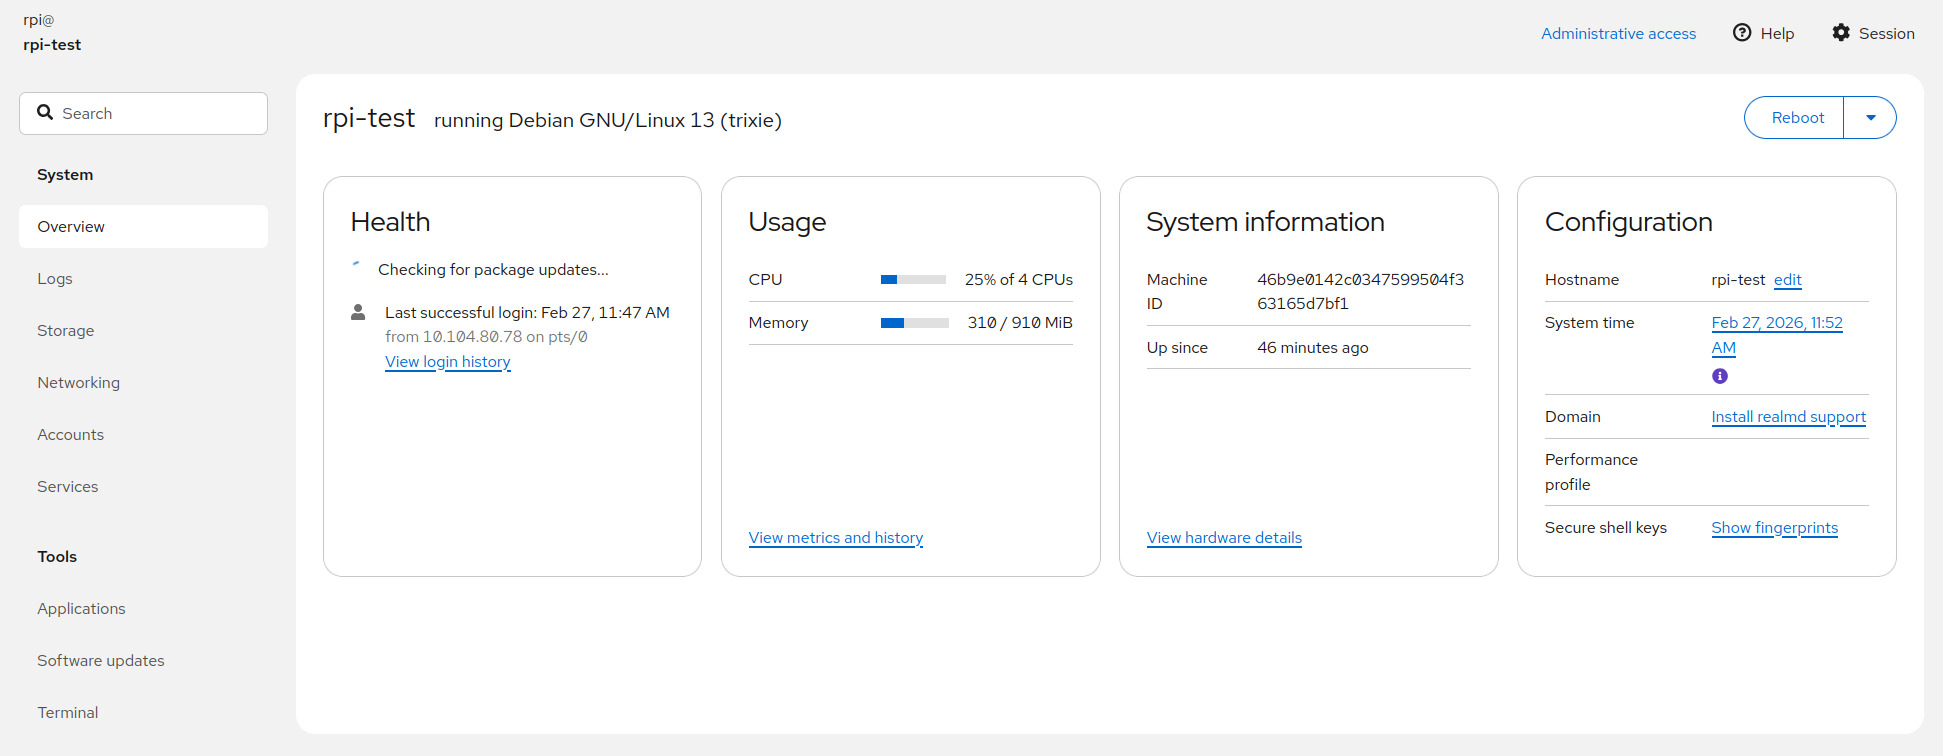
\includegraphics[width=0.9\textwidth]{cockpit}
\end{frame}

\begin{frame}{Cockpit}{Terminal à distance intégré}
    \centering
    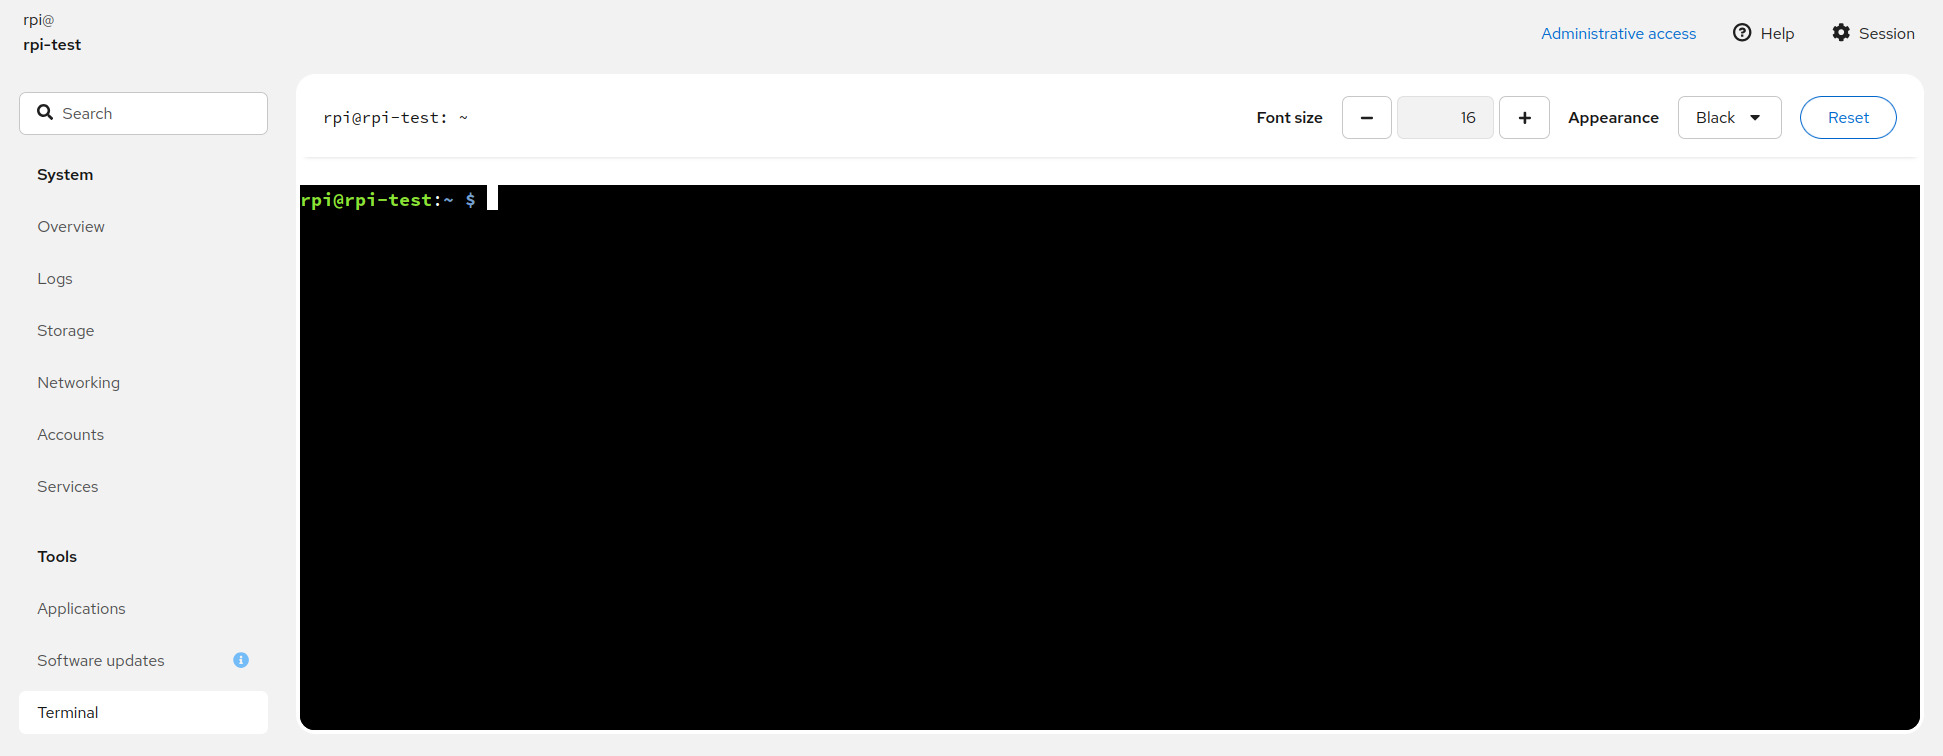
\includegraphics[width=0.9\textwidth]{cockpit_term}
\end{frame}

\begin{frame}{Tmux}
    Garde une session active en arrière plan \(\rightarrow\)
    \alert{parfait pour des mises à jour en SSH}
    \begin{itemize}
        \item \cmd{sudo apt}\args{ install tmux}
        \item \cmd{tmux}: lancer une session tmux
        \item \texttt{Ctrl+B} puis \texttt{D}: détacher la session (elle
              reste active en arrière plan)
        \item \cmd{tmux}\args{ a} (attach): rejoindre la dernière session
    \end{itemize}

    \bigskip
    Exercice:
    \begin{enumerate}
        \item ouvrez un document avec \cmd{less} dans le terminal cockpit
        \item déconnectez internet un instant. \cmd{less} est-il toujours
              ouvert après reconnexion?
        \item répetez l'exercice, mais en utilisant tmux pour préserver votre
              session
        \item détachez la session pendant que \cmd{less} est ouvert, et
              rejoignez-la depuis un terminal SSH, puis depuis le terminal local
    \end{enumerate}
\end{frame}

\begin{frame}{Tmux}{Bonus: plusieurs terminaux en un}
    Tmux est aussi un multiplexeur \(\rightarrow\) plusieurs terminaux dans une
    session!
    \medskip

    \begin{itemize}
        \item \texttt{Ctrl+B} puis \texttt{"} ou \texttt{\%} pour diviser la
              fenêtre en panneaux
        \item \texttt{Ctrl+B} puis flèches pour naviguer entre les
              panneaux
        \item \texttt{Ctrl+B} puis \texttt{C} pour créer une nouvelle fenêtre
        \item \texttt{Ctrl+B} puis \texttt{W} pour naviguer entre les fenêtres
              et
              sessions
        \item \cmd{tmux}\args{ ls} pour lister les sessions tmux en cours
    \end{itemize}

    \bigskip
    Et encore bien d'autres fonctions (voir \texttt{Ctrl+B} puis \texttt{?})

\end{frame}

\end{document}
